\documentclass[a4paper, 10pt]{scrartcl}\usepackage[]{graphicx}\usepackage[]{xcolor}
% maxwidth is the original width if it is less than linewidth
% otherwise use linewidth (to make sure the graphics do not exceed the margin)
\makeatletter
\def\maxwidth{ %
  \ifdim\Gin@nat@width>\linewidth
    \linewidth
  \else
    \Gin@nat@width
  \fi
}
\makeatother

\definecolor{fgcolor}{rgb}{0.345, 0.345, 0.345}
\newcommand{\hlnum}[1]{\textcolor[rgb]{0.686,0.059,0.569}{#1}}%
\newcommand{\hlstr}[1]{\textcolor[rgb]{0.192,0.494,0.8}{#1}}%
\newcommand{\hlcom}[1]{\textcolor[rgb]{0.678,0.584,0.686}{\textit{#1}}}%
\newcommand{\hlopt}[1]{\textcolor[rgb]{0,0,0}{#1}}%
\newcommand{\hlstd}[1]{\textcolor[rgb]{0.345,0.345,0.345}{#1}}%
\newcommand{\hlkwa}[1]{\textcolor[rgb]{0.161,0.373,0.58}{\textbf{#1}}}%
\newcommand{\hlkwb}[1]{\textcolor[rgb]{0.69,0.353,0.396}{#1}}%
\newcommand{\hlkwc}[1]{\textcolor[rgb]{0.333,0.667,0.333}{#1}}%
\newcommand{\hlkwd}[1]{\textcolor[rgb]{0.737,0.353,0.396}{\textbf{#1}}}%
\let\hlipl\hlkwb

\usepackage{framed}
\makeatletter
\newenvironment{kframe}{%
 \def\at@end@of@kframe{}%
 \ifinner\ifhmode%
  \def\at@end@of@kframe{\end{minipage}}%
  \begin{minipage}{\columnwidth}%
 \fi\fi%
 \def\FrameCommand##1{\hskip\@totalleftmargin \hskip-\fboxsep
 \colorbox{shadecolor}{##1}\hskip-\fboxsep
     % There is no \\@totalrightmargin, so:
     \hskip-\linewidth \hskip-\@totalleftmargin \hskip\columnwidth}%
 \MakeFramed {\advance\hsize-\width
   \@totalleftmargin\z@ \linewidth\hsize
   \@setminipage}}%
 {\par\unskip\endMakeFramed%
 \at@end@of@kframe}
\makeatother

\definecolor{shadecolor}{rgb}{.97, .97, .97}
\definecolor{messagecolor}{rgb}{0, 0, 0}
\definecolor{warningcolor}{rgb}{1, 0, 1}
\definecolor{errorcolor}{rgb}{1, 0, 0}
\newenvironment{knitrout}{}{} % an empty environment to be redefined in TeX

\usepackage{alltt}
\usepackage[ngerman]{babel}
% -----------------------------------------------------------------------

% -----------------------------------------------------------------------
%% ------------------------------------------------------------
%% by J.Kruppa on Friday, February 11, 2022 (11:31)
%% \def\mainDir{\Sexpr{exam_path}}
\def\source{/Users/jokruppa/source/tex}
\usepackage[margin=2cm, includefoot]{geometry}
\setlength{\parindent}{0cm}
\usepackage{booktabs}
\usepackage{amsmath}
\usepackage{scalerel,amssymb}
\usepackage{setspace}
\def\csquare{{\Large $\boxtimes$}}
\def\msquare{{\Large $\square$}}
\usepackage[normalem]{ulem}
\usepackage{array}
\usepackage{xcolor}
\usepackage{float}
\usepackage{currfile}
\usepackage{tikz}
\usepackage[nomessages]{fp}

%% beamer defs
\def\lecture{Klausurfragen der Bio Data Science}

%% exam defs
\def\examtitle{\lecture}
\def\exammodule{
\vspace{-1.75cm}  
\begin{graybox}{}
\vspace{2Ex}
\textbf{\large Name:} \rule[0ex]{16.75em}{.4pt}
\hfill \textnormal{\textit{Nicht bestanden:}} \msquare \\[2.5Ex]
\textbf{\large Vorname:} \rule[0ex]{15em}{.4pt} \\[2.5Ex]
\textbf{\large Matrikelnummer:} \rule[0ex]{10.8em}{.4pt}
\hfill Endnote: \rule[0ex]{7em}{.4pt} 
\end{graybox}
\vspace{3Ex}
\phantom{text}
}
\def\examsemester{Sommersemester \& Wintersemester}
\def\examdate{\today}
%% ------------------------------------------------------------
\definecolor{darkblue}{rgb}{0,0,.5}
\definecolor{darkpurple}{rgb}{0.4117, 0.2, 0.4117}
\definecolor{uni}{rgb}{0,0.3137,0.6078}
\definecolor{gray}{gray}{0.7}

\usepackage{tcolorbox}
\definecolor{logo1}{RGB}{0, 158, 227}
\definecolor{gray5}{RGB}{247, 247, 247}
\definecolor{gray2}{RGB}{102, 102, 102}

\newtcolorbox{graybox}[1]{
  colback=gray5,%%red!5!white,
  colframe=gray2,%%red!75!black,
  fonttitle=\bfseries\Large,
  %%valign=center,
  fontupper=\large,
  before skip=10pt plus 2pt,
  after skip=20pt plus 4pt,
  title=#1}

\newtcolorbox{takehomebox}[1]{
  colback=gray5,%%red!5!white,
  colframe=logo1,%%red!75!black,
  fonttitle=\bfseries\Large,
  %%valign=center,
  fontupper=\large,
  before skip=10pt plus 2pt,
  after skip=10pt plus 2pt,
  title=#1}

\def\Rlogo{
\includegraphics[width = 0.5cm]{\string~/Documents/GitHub/exam/img/Rlogo}\;}

\usepackage[scaled=.90]{helvet} 
\usepackage{fancyhdr}
\usepackage{lastpage}
\usepackage{hyperref}
\hypersetup{
    colorlinks=true,       % false: boxed links; true: colored links
    linkcolor=black,          % color of internal links 
    urlcolor=magenta           % color of external links
}
\renewcommand{\familydefault}{\sfdefault}

\title{
\large \exammodule \\[5Ex]
\Huge \examtitle \\[2Ex] 
\Large Hochschule Osnabr{\"u}ck
}
\author{Pr{\"u}fer: Prof. Dr. Jochen Kruppa \\
Fakult{\"a}t f{\"u}r Agrarwissenschaften und Landschaftsarchitektur \\ 
j.kruppa@hs-osnabrueck.de}
\date{Version vom \examdate}

%% ------------------------------------------------------------
%% by J.Kruppa on Tuesday, September 23, 2014 (12:50)
%% Header
\renewcommand{\headrulewidth}{0pt}
\renewcommand{\footrulewidth}{0pt}
\pagestyle{fancy}

\fancyhf{}
\fancyhead[L]{}
\fancyhead[R]{}
\fancyfoot[R]{\thepage}
\fancyfoot[L]{\footnotesize \examtitle}

\fancypagestyle{empty}{
 \fancyhf{}
 \fancyhead[L]{}
 \fancyhead[R]{}
 \fancyfoot[R]{\thepage}
 \fancyfoot[L]{\footnotesize \examtitle}
}

\usepackage{arevtext,arevmath}

\newcommand\Tstrut{\rule{0pt}{2.6ex}}         % = `top' strut
\newcommand\Bstrut{\rule[-0.9ex]{0pt}{0pt}}   % = `bottom' strut
\def\strut{\Tstrut\Bstrut}

% -----------------------------------------------------------------------
\IfFileExists{upquote.sty}{\usepackage{upquote}}{}
\begin{document}
% -----------------------------------------------------------------------
\maketitle
\thispagestyle{empty}
\clearpage
% -----------------------------------------------------------------------
\begin{graybox}{Erlaubte Hilfsmittel f{\"u}r die Klausur}
  \vspace{1Ex}
  \begin{itemize}
  \item Normaler Taschenrechner ohne M{\"o}glichkeit der Kommunikation mit anderen
    Ger{\"a}ten - also ausdr{\"u}cklich kein Handy!
  \item Eine DIN A4-Seite als beidseitig, selbstgeschriebene,
    handschriftliche Formelsammlung - keine digitalen Ausdrucke. 
  \item \textbf{You can answer the questions in English without any
      consequences.}
  \end{itemize}
\end{graybox}
\vfill

\begin{graybox}{Ergebnis der Klausur}
  \vspace{1Ex}
  \begin{itemize}
  \item[] \rule[0ex]{3em}{.4pt}\, von 20\, Punkten sind aus dem Multiple
    Choice Teil erreicht.
  \item[] \rule[0ex]{3em}{.4pt}\, von 64 Punkten sind aus dem Rechen- und
    Textteil erreicht. 
  \item[] \rule[0ex]{3em}{.4pt}\, von 84 Punkten in Summe.
  \item[] Es wird folgender Notenschl{\"u}ssel angewendet.   
  \end{itemize}
  \vspace{1ex}
\begin{center}
  \begin{tabular}[c]{cc}
    \toprule
    \textbf{Punkte}	&	\textbf{Note}	\\
    \midrule
    80.5 - 84.0	&	1,0	\\
    76.0 - 80.0	&	1,3	\\
    72.0 - 75.5	&	1,7	\\
    67.5 - 71.5	&	2,0	\\
    63.5 - 67.0	&	2,3	\\
    59.5 - 63.0	&	2,7	\\
    55.0 - 59.0	&	3,0	\\
    51.0 - 54.5	&	3,3	\\
    46.5 - 50.5	&	3,7	\\
    42.0 - 46.0	&	4,0	\\
    \bottomrule
  \end{tabular}
\end{center}
  \vspace{1ex}
\begin{itemize}
\item[] Es ergibt sich eine Endnote von \rule[0ex]{4em}{.4pt}.
\end{itemize}
  \vspace{1Ex}
\end{graybox}

% -----------------------------------------------------------------------
\newpage
% -----------------------------------------------------------------------

\begin{graybox}{Multiple Choice Aufgaben}
  \begin{itemize}
  \item Pro Multipe Choice Frage ist \emph{genau} eine Antwort richtig.
  \item \textbf{{\"U}bertragen Sie Ihre Kreuze in die Tabelle auf
      dieser Seite.}
  \item Es werden nur Antworten ber{\"u}cksichtigt, die in dieser Tabelle
    angekreuzt sind!
  \end{itemize}

\begin{center}
  \large
  \begin{tabular}{|r|c|c|c|c|c||c|}
    \hline
    & \textbf{A} & \textbf{B} & \textbf{C} & \textbf{D} & \textbf{E} & $\boldsymbol{\checkmark}$\strut\\
    \hline
    1 Aufgabe &   &   &   &   &   & \strut\\
    \hline
    2 Aufgabe &   &   &   &   &   & \strut\\
    \hline
    3 Aufgabe &   &   &   &   &   & \strut\\
    \hline
    4 Aufgabe &   &   &   &   &   & \strut\\
    \hline
    5 Aufgabe &   &   &   &   &   & \strut\\
    \hline
    6 Aufgabe &   &   &   &   &   & \strut\\
    \hline
    7 Aufgabe &   &   &   &   &   & \strut\\
    \hline
    8 Aufgabe &   &   &   &   &   & \strut\\
    \hline
    9 Aufgabe &   &   &   &   &   & \strut\\
    \hline
    10 Aufgabe &   &   &   &   &   & \strut\\
    \hline
  \end{tabular}
\end{center}

\begin{itemize}
\item Es sind \rule[0ex]{2em}{.4pt}\, von 20 Punkten erreicht worden.
\end{itemize}
\end{graybox}

\vfill

\begin{graybox}{Rechen- und Textaufgaben}
  \begin{itemize}
  \item Die Tabelle wird vom Dozenten ausgef{\"u}llt.
  \end{itemize}
  \begin{center}
    \large
    \begin{tabular}{|l|c|c|c|c|c|c|c|}
      \hline
      \textbf{Aufgabe} & 11 & 12 & 13 & 14 & 15 & 16 & 17 \strut\\
      \hline
      \textbf{Punkte} & 
      \hspace{1Ex}\Large\textcolor{gray!70}{12}\hspace{1Ex}  & 
      \hspace{1Ex}\Large\textcolor{gray!70}{6}\hspace{1Ex}  & 
      \hspace{1Ex}\Large\textcolor{gray!70}{7}\hspace{1Ex}  & 
      \hspace{1Ex}\Large\textcolor{gray!70}{10}\hspace{1Ex}  & 
      \hspace{1Ex}\Large\textcolor{gray!70}{11}\hspace{1Ex}  & 
      \hspace{1Ex}\Large\textcolor{gray!70}{8}\hspace{1Ex}  & 
      \hspace{1Ex}\Large\textcolor{gray!70}{10}\hspace{1Ex} \strut\\
      \hline
  \end{tabular}
\end{center}
\begin{itemize}
\item Es sind \rule[0ex]{2em}{.4pt}\, von 64 Punkten erreicht worden.
\end{itemize}
\end{graybox}

% -----------------------------------------------------------------------
\clearpage
% -----------------------------------------------------------------------

\section{Aufgabe \hfill (2 Punkte)}



Sie haben folgende unadjustierten p-Werte gegeben: 0.89, 0.34, 0.001, 0.21 und 0.03. Sie adjustieren die p-Werte nach
Bonferroni. Welche Aussage ist richtig?



\begin{enumerate}
\item [\textbf{A} \msquare] Nach der Bonferroni-Adjustierung ergeben sich die adjustierten p-Werte von 0.178, 0.068, 2e-04, 0.042 und 0.006. Die adjustierten p-Werte werden zu einem $\alpha$-Niveau von 1\% verglichen.
\item [\textbf{B} \msquare] Nach der Bonferroni-Adjustierung ergeben sich die adjustierten p-Werte von 1, 1, 0.005, 1 und 0.15. Die adjustierten p-Werte werden zu einem $\alpha$-Niveau von 1\% verglichen.
\item [\textbf{C} \msquare] Nach der Bonferroni-Adjustierung ergeben sich die adjustierten p-Werte von 1, 1, 0.005, 1 und 0.15. Die adjustierten p-Werte werden zu einem $\alpha$-Niveau von 5\% verglichen.
\item [\textbf{D} \msquare] Nach der Bonferroni-Adjustierung ergeben sich die adjustierten p-Werte von 0.178, 0.068, 2e-04, 0.042 und 0.006. Die adjustierten p-Werte werden zu einem $\alpha$-Niveau von 5\% verglichen.
\item [\textbf{E} \msquare] Nach der Bonferroni-Adjustierung ergeben sich die adjustierten p-Werte von 4.45, 1.7, 0.005, 1.05 und 0.15. Die adjustierten p-Werte werden zu einem $\alpha$-Niveau von 5\% verglichen.
\end{enumerate} 

\section{Aufgabe \hfill (2 Punkte)}



Der Datensatz \texttt{PlantGrowth} enth{\"a}lt das Gewicht von Pflanzen, die
unter einer Kontrolle und zwei verschiedenen Behandlungsbedingungen erzielt
wurden. Nach der Berechnung einer einfaktoriellen ANOVA ergibt sich ein
$\eta^2 = 0.2$. Welche Aussage ist richtig?



\begin{enumerate}
\item [\textbf{A} \msquare] Das $\eta^2$ ist die Korrelation der ANOVA. Mit der Ausnahme, dass 0 der beste Wert ist.
\item [\textbf{B} \msquare] Das $\eta^2$ ist ein Wert f{"u}r die G{"u}te der ANOVA. Je kleiner desto besser. Ein $\eta^2$ von 0 bedeutet ein perfektes Modell mit keiner Abweichung. Die Varianz ist null.
\item [\textbf{C} \msquare] Das $\eta^2$ beschreibt den Anteil der Varianz, der von den Behandlungsbedingungen erkl{"a}rt wird. Das $\eta^2$ ist damit mit dem $R^2$ aus der linearen Regression zu vergleichen.
\item [\textbf{D} \msquare] Das $\eta^2$ beschreibt den Anteil der Varianz, der von den Behandlungsbedingungen nicht erkl{"a}rt wird. Somit der Rest an nicht erkl{"a}rbarer Varianz.
\item [\textbf{E} \msquare] Die Berechnung von $\eta^2$ ist ein Wert f{"u}r die Interaktion.
\end{enumerate} 

\section{Aufgabe \hfill (2 Punkte)}

Die folgende Abbildung enth{\"a}lt die Daten aus einer Studie zur
Bewertung der Wirkung von Vitamin C auf das Zahnwachstum bei
Meerschweinchen. Der Versuch wurde an 60 Schweinen durchgef{\"u}hrt, wobei
jedes Tier eine von drei Vitamin-C-Dosen (0.5, 1 und 1.5 mg/Tag) {\"u}ber eine
von zwei Verabreichungsmethoden mit Orangensaft (OJ)  oder
Ascorbins{\"a}ure (VC) erhielt. 



{\centering 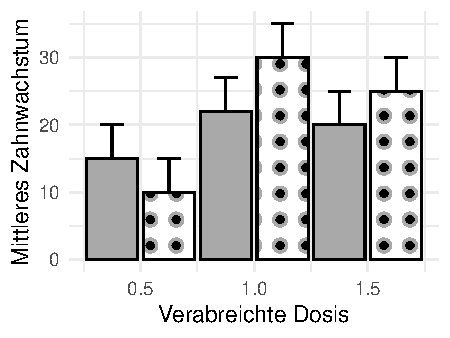
\includegraphics[width=\maxwidth]{img/mc-anova-02-a-1} 

}




Welche Aussage ist richtig im Bezug auf eine zweifaktorielle ANOVA?



\begin{enumerate}
\item [\textbf{A} \msquare] Keine Interaktion liegt vor. Die Geraden scheiden sich und laufen nicht parallel.
\item [\textbf{B} \msquare] Eine starke Interaktion ist zu erwarten. Die Geraden schneiden sich und die Abst{"a}nde sind nicht gleichbleibend.
\item [\textbf{C} \msquare] Eine starke Interaktion liegt vor. Die Geraden laufen parallel und schneiden sich nicht.
\item [\textbf{D} \msquare] Eine leichte Interaktion ist zu erwarten. Die Geraen schneiden sich noch nicht, aber die Abst{"a}nde unterscheiden sich stark.
\item [\textbf{E} \msquare] Keine Interaktion ist zu erwatzen. Die Geraden der Verabreichungsmethode laufen parallel und mit {"a}hnlichen Abst{"a}nden.
\end{enumerate} 

\section{Aufgabe \hfill (2 Punkte)}

Eine einfaktorielle ANOVA berechnet eine Teststatistik um zu die Nullhypothese abzulehnen. Welche Aussage {\"u}ber die Teststatistik der ANOVA ist richtig?



\begin{enumerate}
\item [\textbf{A} \msquare] Die ANOVA berechnet die F-Statistik indem die MS der Behandlung durch die MS des Fehlers geteilt werden. Wenn die F-Statistik sich der 0 ann{"a}hert kann die Nullhypothese nicht abgelehnt werden.
\item [\textbf{B} \msquare] Die ANOVA berechnt die F-Statistik aus den SS Behandlung geteilt durch die SS Fehler.
\item [\textbf{C} \msquare] Die ANOVA berechnet die T-Statistik aus der Multiplikation der MS Behandlung mit der MS der Fehler. Wenn die F-Statistik genau 0 ist, kann die Nullhypothese abgelehnt werden.
\item [\textbf{D} \msquare] Die ANOVA berechnet die T-Statistik indem den Mittelwertsunterschied der Gruppen simultan durch die Standardabweichung der Gruppen teilt. Wenn die T-Statistik h{"o}her als 1.96 ist, kann die Nullhypothese abgelehnt werden.
\item [\textbf{E} \msquare] Die ANOVA berechnet die F-Statistik indem die MS des Fehlers durch die MS der Behandlung geteilt werden. Wenn die F-Statistik sich der 1 ann{"a}hert kann die Nullhypothese nicht abgelehnt werden.
\end{enumerate} 

\section{Aufgabe \hfill (2 Punkte)}




Sie haben das abstrakte Modell $Y \sim X$ mit $X$ als Faktor mit zwei
Leveln vorliegen. Welche Aussage {\"u}ber $n_1 = n_2$ ist richtig?



\begin{enumerate}
\item [\textbf{A} \msquare] Es handelt sich um ein unbalanciertes Design
\item [\textbf{B} \msquare] Es handelt sich um ein balanciertes Design.
\item [\textbf{C} \msquare] Es liegt Varianzhetrogenit{"a}t vor.
\item [\textbf{D} \msquare] Es liegt Varianzhomogenit{"a}t vor.
\item [\textbf{E} \msquare] Es handelt sich um abh{"a}ngige Beobachtungen.
\end{enumerate} 

\section{Aufgabe \hfill (2 Punkte)}

Die Mindestanzahl an Beobachtungen f{\"u}r eine Zelle der Vierfeldertafel bei
der Nutzung eines Chi-Quadrat-Testes ist...



\begin{enumerate}
\item [\textbf{A} \msquare] 5 Beobachtungen
\item [\textbf{B} \msquare] 10 Beobachtungen
\item [\textbf{C} \msquare] 1 Beobachtung
\item [\textbf{D} \msquare] 0 Beobachtungen
\item [\textbf{E} \msquare] 2 Beobachtungen
\end{enumerate} 

\section{Aufgabe \hfill (2 Punkte)}




Welche Aussage {\"u}ber den Korrelationskoeffizienten nach Pearson
ist richtig?



\begin{enumerate}
\item [\textbf{A} \msquare] Der Korrelationskoeffizienten nach Pearson wird genutzt, wenn das Outcome Y normalverteilt ist. Der Korrelationskoeffizienten liegt zwischen 0 und 1.
\item [\textbf{B} \msquare] Der Korrelationskoeffizienten nach Pearson wird genutzt, wenn der Korrelationskoeffizienten zwischen -1 und 1 liegt. Dann sind die Residuen normalverteilt.
\item [\textbf{C} \msquare] Der Korrelationskoeffizienten nach Pearson wird genutzt, wenn das Outcome Y normalverteilt ist. Der Korrelationskoeffizienten liegt zwischen -1 und 1.
\item [\textbf{D} \msquare] Der Korrelationskoeffizienten nach Pearson wird genutzt, wenn das Outcome Y nicht normalverteilt ist. Der Korrelationskoeffizienten liegt zwischen -1 und 1.
\item [\textbf{E} \msquare] Der Korrelationskoeffizienten nach Pearson wird genutzt, wenn das Outcome Y nicht normalverteilt ist. Der Korrelationskoeffizienten liegt zwischen 0 und 1.
\end{enumerate} 

\section{Aufgabe \hfill (2 Punkte)}




Berechnen Sie den Mittelwert und Standardabweichung von $y$ mit 6, 9, 6, 6 und 14.



\begin{enumerate}
\item [\textbf{A} \msquare] Es ergibt sich 8.2 +/- 12.2
\item [\textbf{B} \msquare] Es ergibt sich 8.2 +/- 1.745
\item [\textbf{C} \msquare] Es ergibt sich 8.2 +/- 3.49
\item [\textbf{D} \msquare] Es ergibt sich 7.2 +/- 6.1
\item [\textbf{E} \msquare] Es ergibt sich 9.2 +/- 1.745
\end{enumerate} 

\section{Aufgabe \hfill (2 Punkte)}




Berechnen Sie den Median, das $1^{st}$ Quartile sowie das $3^{rd}$ Quartile von $y$ mit 25, 17, 21, 30, 6, 1, 33, 6, 20, 15 und 51.



\begin{enumerate}
\item [\textbf{A} \msquare] Es ergibt sich 20 [6, 30]
\item [\textbf{B} \msquare] Es ergibt sich 20 [7, 31]
\item [\textbf{C} \msquare] Es ergibt sich 20 +/- 6
\item [\textbf{D} \msquare] Es ergibt sich 20 +/- 6
\item [\textbf{E} \msquare] Es ergibt sich 20 +/- 30
\end{enumerate} 

\section{Aufgabe \hfill (2 Punkte)}

Welche Aussage {\"u}ber Cook's d und Cohen's d ist richtig? 



\begin{enumerate}
\item [\textbf{A} \msquare] Wir nutzen Cook's d um Outlier in den Daten zu finden und Cohen's d um einen nicht standardisierten Effektsch{"a}tzer f{"u}r Gruppenvergeliche zu erhalten.
\item [\textbf{B} \msquare] Wir nutzen Cook's d um Outlier in den Daten zu finden und Cohen's d um standardisierte Outlier f{"u}r Gruppenvergeliche zu erhalten.
\item [\textbf{C} \msquare] Wir nutzen Cohen's d um Outlier in den Daten zu finden und Cook's d um einen standardisierten Effektsch{"a}tzer f{"u}r Gruppenvergeliche zu erhalten.
\item [\textbf{D} \msquare] Wir nutzen Cook's d um Outlier in den Daten zu finden und Cohen's d um einen standardisierten Effektsch{"a}tzer f{"u}r Gruppenvergeliche zu erhalten.
\item [\textbf{E} \msquare] Wir nutzen Cook's d um Outlier in den Daten zu finden. Cohen's d findet auch Outlier, ist aber ein veraltetetes Konzept in der Statistik.
\end{enumerate}
% -----------------------------------------------------------------------

\section{Aufgabe \hfill (10 Punkte)}

\textit{Geben Sie grunds{\"a}tzlich Formeln und Rechenweg zur L{\"o}sung der
  Teilaufgaben mit an!} \\[1Ex]

%% --------------------------------------------------------------------
\hfill\href{https://youtu.be/sBlSc_eJbnw}{
\includegraphics[width =
  2cm]{img/youtube}}\\[1Ex]
%% --------------------------------------------------------------------


Sie haben folgende Zahlenreihe $y$ vorliegen
$y = \{17, 8, 16, 16, 14, 17, 13\}$. Berechnen Sie folgende
deskriptive Ma{\ss}zahlen. 



\begin{enumerate}
\item Die Varianz \textbf{(2 Punkte)}
\item Das 1st Quartile \textbf{(2 Punkte)}
\item Den Interquartileabstand \textbf{(2 Punkte)}
\item Das 3rd Quartile \textbf{(2 Punkte)}
\item Die Standardabweichung \textbf{(2 Punkte)}
\end{enumerate}
 
\clearpage
% -----------------------------------------------------------------------

\section{Aufgabe \hfill (8 Punkte)}

\textit{Geben Sie grunds{\"a}tzlich Formeln und Rechenweg zur L{\"o}sung der
  Teilaufgaben mit an!} \\[1Ex]

%% --------------------------------------------------------------------
\hfill\href{https://youtu.be/oMdtYbDInYE}{
\includegraphics[width =
  2cm]{img/youtube}}\\[1Ex]
%% --------------------------------------------------------------------

Sie haben folgende Zahlenreihe $y$ vorliegen
$y = \{11, 15, 15, 15, 15, 13, 17\}$.

\begin{enumerate}
\item Visualisieren Sie den Mittelwert von $y$ in der untenstehenden
  Abbildung! \textbf{(4 Punkte)}
\item Beschriften Sie die $Y$ und $X$-Achse entsprechend! \textbf{(2 Punkte)}
\item F{\"u}r die Berechnung der Varianz wird der Abstand der einzelnen Werte $y_i$
  zum Mittelwert $\bar{y}$ quadriert. Warum muss der Abstand, $y_i -
  \bar{y}$, in der Varianzformel quadriert werden?
  Erkl{\"a}ren Sie den Zusammenhang unter Ber{\"u}cksichtigung der Abbildung!
  \textbf{(2 Punkte)}  
\end{enumerate}



{\centering 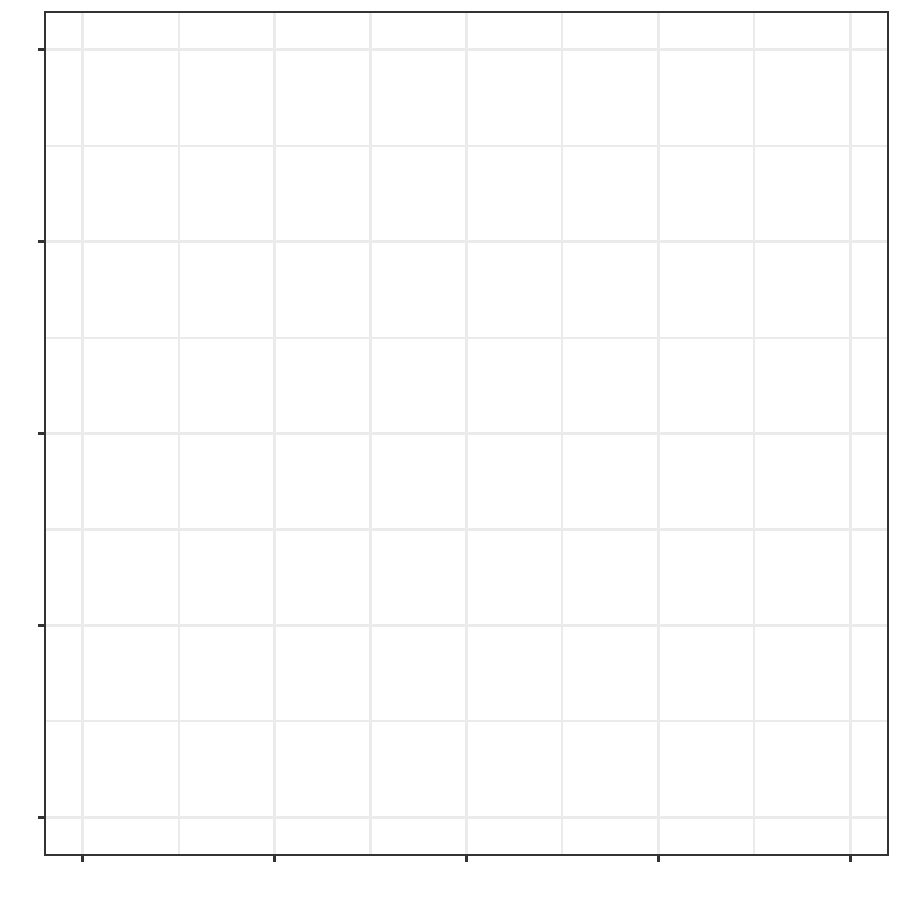
\includegraphics[width=\maxwidth]{img/desc-01-1} 

}


 
\clearpage
% -----------------------------------------------------------------------

\section{Aufgabe \hfill (7 Punkte)}

\textit{Geben Sie grunds{\"a}tzlich Formeln und Rechenweg zur L{\"o}sung der
  Teilaufgaben mit an!} \\[1Ex]

%% --------------------------------------------------------------------
\hfill\href{https://youtu.be/vXnLttRL_VI}{
\includegraphics[width =
  2cm]{img/youtube}}\\[1Ex]
%% --------------------------------------------------------------------

Nach einem Gew{\"a}chshausexperiment mit drei Bew{\"a}sserungstypen ($low$, $mid$
und $high$) ergibt sich die folgende Datentabelle mit dem gemessenen
Frischgewicht (\textit{freshmatter}).

\begin{table}[!h]
\centering
\begin{tabular}{cc}
\toprule
water\_type & freshmatter\\
\midrule
low & 15\\
low & 10\\
low & 16\\
mid & 26\\
mid & 28\\
\addlinespace
mid & 25\\
low & 14\\
high & 8\\
high & 10\\
low & 13\\
\addlinespace
high & 9\\
\bottomrule
\end{tabular}
\end{table}



\begin{enumerate}
\item Zeichnen Sie in \textit{einer} Abbildung die Barplots f{\"u}r die
  Bew{\"a}sserungstypen! Beschriften Sie die Achsen entsprechend!  \textbf{(4
    Punkte)}
\item Beschriften Sie \textit{einen} Barplot mit den g{\"a}ngigen
  statistischen Ma{\ss}zahlen! \textbf{(2 Punkte)}
\item Wenn Sie \textit{keinen Effekt} zwischen der Bew{\"a}sserungstypen
  erwarten w{\"u}rden, wie sehen dann die Barplots aus? \textbf{(1 Punkt)}
\end{enumerate} 
\clearpage
% -----------------------------------------------------------------------

\section{Aufgabe \hfill (6 Punkte)}

\textit{Geben Sie grunds{\"a}tzlich Formeln und Rechenweg zur L{\"o}sung der
  Teilaufgaben mit an!} \\[1Ex]

%% --------------------------------------------------------------------
\hfill\href{https://youtu.be/MiD42k4l5Ag}{
\includegraphics[width =
  2cm]{img/youtube}}\\[1Ex]
%% --------------------------------------------------------------------



\begin{enumerate}
\item Skizieren Sie in die unten stehenden, freien Abbildungen die
  Verteilungen, die sich nach der Abbildungs{\"u}berschrift ergeben! \textbf{(4
    Punkte)}
\item Achten Sie auf die entsprechende Skalierung der beiden Verteilungen
  in der ersten Abbildung! \textbf{(2 Punkte)}
\end{enumerate}



{\centering 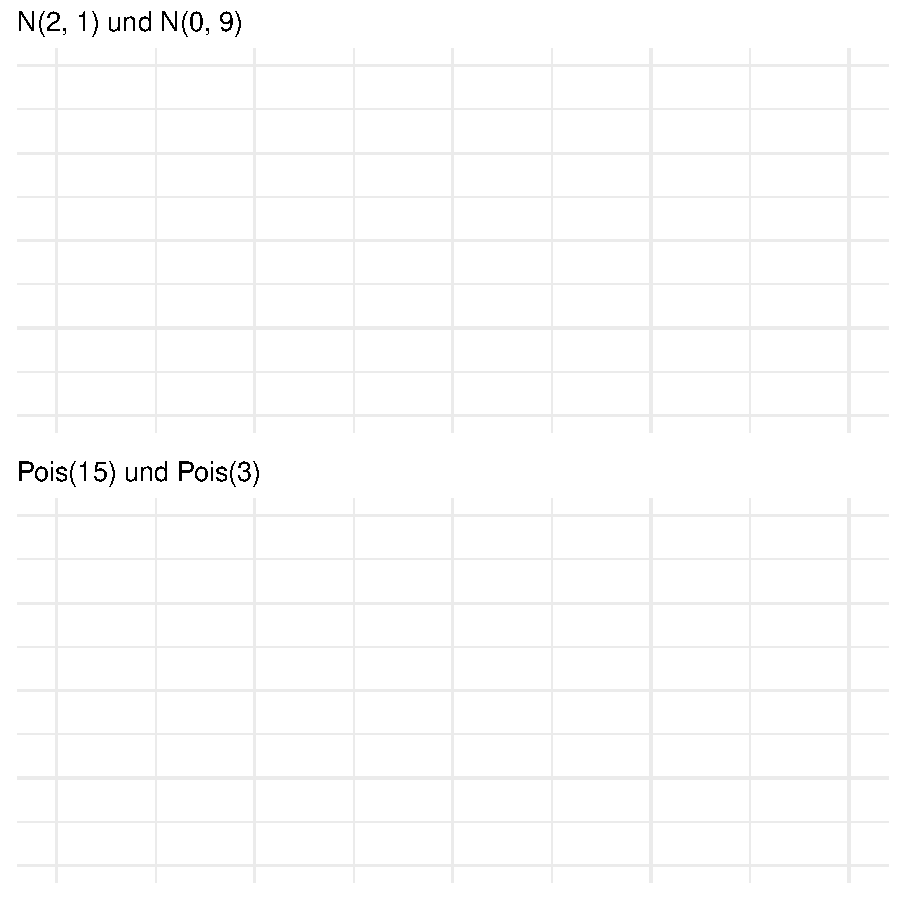
\includegraphics[width=\maxwidth]{img/histogram-01-1} 

}



 
\clearpage
% -----------------------------------------------------------------------

\section{Aufgabe \hfill (6 Punkte)}

\textit{Geben Sie grunds{\"a}tzlich Formeln und Rechenweg zur L{\"o}sung der
  Teilaufgaben mit an!} \\[1Ex]

%% --------------------------------------------------------------------
\hfill\href{https://youtu.be/ZrJhn2wPbq4}{
\includegraphics[width =
  2cm]{img/youtube}}\\[1Ex]
%% --------------------------------------------------------------------



\begin{enumerate}
\item Skizieren Sie $4$ Normalverteilungen \textit{in einer
    Abbildung} mit $\bar{y}_1 \neq \bar{y}_2 \neq \bar{y}_3 \neq \bar{y}_4$ und $s_1 \neq s_2 \neq s_3 \neq s_4$! \textbf{(2 Punkte)}
\item Beschriften Sie die Normalverteilungen mit den entsprechenden
  Parametern! \textbf{(2 Punkte)}
\item Liegt Varianzhomogenit{\"a}t oder Varianzheterogenit{\"a}t vor? Begr{\"u}nden Sie
  Ihre Antwort! \textbf{(2 Punkte)}
\end{enumerate}

 
\clearpage
% -----------------------------------------------------------------------

\section{Aufgabe \hfill (6 Punkte)}

\textit{Geben Sie grunds{\"a}tzlich Formeln und Rechenweg zur L{\"o}sung der
  Teilaufgaben mit an!} \\[1Ex]

%% --------------------------------------------------------------------
\hfill\href{https://youtu.be/aXvxGC4YLqk}{
\includegraphics[width =
  2cm]{img/youtube}}\\[1Ex]
%% --------------------------------------------------------------------



Nach einem Experiment z{\"a}hlen Sie folgende Anzahl an L{\"a}sionen auf den
Bl{\"a}ttern von Sonnenblumen nach einer durchgestandenen Infektion. 

\begin{center}
$4, 6, 2, 3, 4, 9, 2, 6, 4, 5, 5, 4$
\end{center}

\begin{enumerate}
\item Zeichen Sie ein Histogramm um die Verteilung der Daten zu visualiseren! (\textbf{3 Punkte})
\item Beschriften Sie die Achsen der Abbildung! (\textbf{2 Punkte})
\item Erg{\"a}nzen Sie die relativen H{\"a}ufigkeiten in der Abbildung! \textbf{(1
    Punkt)}  
\end{enumerate}

 
\clearpage
% -----------------------------------------------------------------------

\section{Aufgabe \hfill (8 Punkte)}

\textit{Geben Sie grunds{\"a}tzlich Formeln und Rechenweg zur L{\"o}sung der
  Teilaufgaben mit an!} \\[1Ex]

%% --------------------------------------------------------------------
\hfill\href{https://youtu.be/ORHSPTCdfeY}{
\includegraphics[width =
  2cm]{img/youtube}}\\[1Ex]
%% --------------------------------------------------------------------



Nach einem Experiment z{\"a}hlen Sie folgende Trockengewichte von Sonnenblumen nach einer durchgestandenen Infektion. 

\begin{center}
$7.9, 7.5, 8.3, 8.4, 9.5, 16.5, 11, 9.8, 10.3, 6.3, 12.4, 12.7$
\end{center}

\begin{enumerate}
\item Zeichen Sie ein Histogramm um die Verteilung der Daten zu
  visualiseren! (\textbf{3 Punkte})
 \item Erl{\"a}utern Sie Ihr Vorgehen um ein Histogramm f{\"u}r kontinuierliche
  Daten zu zeichnen!  (\textbf{2 Punkte})
\item Beschriften Sie die Achsen der Abbildung! (\textbf{2 Punkte})
\item Erg{\"a}nzen Sie die relativen H{\"a}ufigkeiten in der Abbildung! \textbf{(1
    Punkt)}  
\end{enumerate}

 
\clearpage
% -----------------------------------------------------------------------

% -----------------------------------------------------------------------
\end{document}
% -----------------------------------------------------------------------


  
